\chapter{Fresnel Zones}
\label{fres_zone}


Fresnel zone \citep{Fres1} \citep{Fres2} calculations gives a mean to calculate on how to avoid the interference from the strongest radio signals that are not direct line signals. This can be caused by reflections of obstacles, these reflected signals will have a different phase and when added with the direct line signal, may cause power loss. There are an infinite amount of Fresnel zones, and all will impact the direct line signal.  %Where these Fresnel zones are created, where there exists and infinite amount of them.   %and will make the reflected signals to be out of phase. 

%the impact of out of phase signals caused by reflections of obstacles, on the signal as whole from the transmitter to the receiver.

%are used to calculate the reflections and diffraction loss between an transmitter and a receiver. 
In terms of a radio signal travelling from a transmitter to a receiver it can travel along different paths. It can travel directly without any reflection, %which is the most ideal%. 
or it could reflect of the ground and thereby carry on to the receiver, or it could be reflected by a hill, and carry on to the receiver. %which is not desirable, but in some circumstances inevitable. 
These reflections can cause a signal loss from the transmitter to the receiver. The receiver does not differentiate between the reflected and the direct line signals, and therefore it will consider both the reflected and the direct line signal as the intended signal \citep{Fres2}. It is important to notice that there will be a phase shift of $180^{\circ}$, if the wave is linearly polarized and hits a surface that is parallel to the waves polarization. 

%It is important to note that the reflection itself will create an change in phase up to $180^{\circ}$, the lower the incidence angle the closer to $180^{\circ}$ \citep{Fres3}.  %So therefore when calculating the Fresnel zones it will take into consideration the reflections and diffraction loss, and will 

If these signals reflect of an obstacle and are out of phase with the direct line signals, they may end up having phase cancellation effect which could end up minimizing the power of the signals. For example two identical radio signals out of phase will cancel each other out and therefore no signal will be received, by the receiver. So therefore when calculating Fresnel zones it must be taken into consideration which out of phase signals from reflections have the most effect on the direct line signal, and make sure that it does not lose a lot of power. 

There are an infinite amount of Fresnel zones, but the most important Fresnel zone is the first one. This is due to that the strongest signals are the ones that are closets to the direct line signal %which travels without any reflections and will have the same power through the path, 
and they always lie in the first Fresnel Zone.  
Which also means that the second, third and so on Fresnel zones are further and further from the Direct signal and obstacles in these will have a lesser impact \citep{introRF}. This can be seen on the following Figure, which is illustrated with 2 Fresnel zones, Fresnel zone 1 and 2:
\begin{figure}[H]
\centering
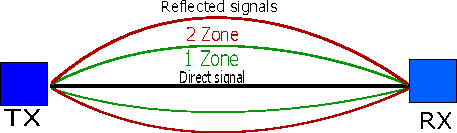
\includegraphics[width=0.6\textwidth]{fresnel_ill_1.pdf}
\caption{Illustration of the First and Second Fresnel zone, along with the Direct signal travelling from the Transmitter TX to the Receiver RX}
\label{dijdk}
\end{figure}

As it can be seen the first Fresnel zone is closets to the direct signal and will have the strongest cancelling effect, if not taken into consideration. It has the least amount of delay in the reflected signal of the first Fresnel zone as it travels least from the transmitter to the receiver. Inside the first Fresnel zone phase delay due to increase in path distance of the reflected wave are $0^\circ$-$90^\circ$, when remembering the phase change done by the reflection itself that means the signal is $180^\circ$-$270^\circ$ out of phase in total. When the reflected signal then interfere with the direct signal destructive interference occur. In terms of the second Fresnel zone, it creates longer phase delay, in total between $270^\circ$ to $450^\circ$ out of phase. This become constructive interference. The phase cancelling effect in even numbered Fresnel zones are good while odd numbered zones are bad. A rule of thumb in terms of the first Fresnel zone is that \textit{$60\%$ of the first Fresnel zone must be cleared of any obstacles}, as this reduces the destructive interference significantly \citep{introRF}\citep{Fres2}. 
\\
\\


\textbf{Fresnel zone 1}
\\
\\
As mentioned $60\%$ of the first Fresnel zone must be cleared of objects, an illustration of this can be seen on the following Figure:
\begin{figure}[H]
\centering
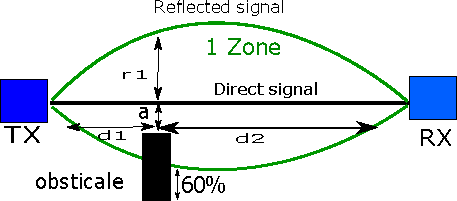
\includegraphics[width=0.6\textwidth]{fresnel_ill_obs.pdf}
\caption{Illustration of the First Fresnel zone cleared $60\%$, with an building representing the obstacle}
\label{dijdk1}
\end{figure}


The obstacle on the Figure above could illustrate a building where $d_{1}$ is the distance from the transmitter $TX$ to the building while $d_{2}$ is the distance from the receiver $RX$ to the building. The radius of the first Fresnel zone is $r_1$. The distance from the direct signal to the obstacle is $a$. 
With this in mind the rule of thumb states that $a > 0.6\cdot r_1$. 


%The obstacle on the Figure above could illustrate a building where $d_{1}$ is the distance from the transmitter $TX$ to the building while $d_{2}$ is the distance from the receiver $RX$ to the building. While $a$ is the center line of sight, which means that there is a obstacle free direct view to the receiver, for the signal to travel. So the building must not be closer than $60\%$ of the measured $r1$ which is the radius of the first Fresnel zone from the center line of sight $a$, to fulfil the requirement of $60\%$ clearance, in the first Fresnel zone. Which in other words means that there must be $60\%$ line of sight, according to the radius of the first Fresnel zone, which represents the impact of the reflected signal ,to travel with the direct signal. %Where the $60\%$ is calculated according to the radius of the first Fresnel zone.

 %where from the center point to the receiver $RX$ shall represent the $60\%$. 

%So $c$ is $r1 \cdot 0.6$



\textbf{Fresnel Zone calculations}

The general equation for calculating the Fresnel zone radius at any point a in between the endpoints is given as \citep{introRF}:

\begin{equation}
F_{n} = \sqrt{\frac{n \lambda d_{1} d_{2}}{d_{1}+d_{2}}}
\label{fres:eq1}
\end{equation}

\begin{where}
\va{$F_{n}$}{The $n^{th}$ Fresnel Zone radius}{m}
\va{$d_{1}$}{The distance of $a$ from TX}{m}
\va{$d_{2}$}{The distance of $a$ from RX}{m}
\va{$\lambda$}{The wavelength of the signal}{m}
\end{where}

A conservative calculation of the $60\%$ rule of thumb is to use the maximum radius of the first Fresnel zone to calculate maximum obstacle heights. %With the maximum radius of the first Fresnel zone and the obstacle height, the maximum obstacle height can be calculated, with respect to $60\%$ clearance. %so that the Transmitter and the Receiver can have LOS, and the first Fresnel zone will be $60\%$ cleared. 


The wavelength $\lambda$ can be expressed as:

\begin{equation}
\lambda = \frac{c}{f}
\label{fres:eq2}
\end{equation}

\begin{where}
\va{$c$}{The speed of light in a vacuum}{3$\cdot$$10^{8}$$ms^{-1}$}
\va{$f$}{Signal frequency}{$Hz$}
\end{where}




%While mostly the interest is the maximum radius of the Fresnel zone 


The maximum radius is found at the point where $d_{1} = d_{2}$. Then by using this as well as setting $n=1$ as it is the first Fresnel zone. An expression for the maximum radius can be found and if \autoref{fres:eq2} is inserted into \autoref{fres:eq1} that yields:


\begin{equation}
r = 8.67 \cdot \sqrt{\frac{D}{f}}
\label{fres:eq3}
\end{equation}

\begin{where}
\va{$D$}{Total distance = $d_{1} + d_{2}$}{km}
\va{$f$}{Signal frequency}{GHz}
\end{where}

As an example to calculate the clearance radius of the first Fresnel zone of two antennas operating 5.5 GHz, with a distance $D$ of 500m. The 60$\%$ clearance radius $a$ is given as:

\begin{equation}
a = 0.60\cdot8.67 \cdot \sqrt{\frac{0.50}{5.5}} = 1.57 m
\label{fres:eq_ex}
\end{equation}

Then by subtracting the antenna height form $a$, the maximum obstacle height with respect to the 60$\%$ clearance can be calculated. So if the the antenna height is 10m, then by subtracting 10m-1.57m we get 8.43 m, which is the maximum obstacle height.  %So to compare with the Figure illustrated with the obstacle \ref{dijdk}, the 10m is the height of the TX and RX where the antennas placed. While the the 60$\%$ clear Fresnel zone maximum radius $r$ is calculated to be 2.02 m. So
%\newpage
%\textbf{Earth curvature}



%http://www.4gon.co.uk/solutions/technical_fresnel_zones.php

%http://radiomobile.pe1mew.nl/?Calculations:Propagation_calculation:Fresnel_zones

%http://www.zytrax.com/tech/wireless/fresnel.htm

%https://s.campbellsci.com/documents/au/technical-papers/line-of-sight-obstruction.pdf

%must lie in the direct line, 

%which is always in the first Fresnel zone. 

%In order to get the maximum signal strength, the effect of the out of phase signals must be minimised.         




%%An illustration of Fresnel zones can be seen on the following Figure:
 




%Fresnel zone radius describes this reflection in relation to the overall path of the signal, which means the whole path from the transmitter to the receiver is taken into account, with the reflections. A reflection can happen anywhere in the path between the transmitter and the receiver.
%\\
%\\
%When a signal is reflected two things can happen:

%\begin{itemize}
%\item The phase of the signal reverses and the signal changes in phase by $180\deg$
%\item As the signal is being reflected and thereby not going in a direct line, it will travel further. Therefore the signal is shifted further in phase, by the difference in path length 
%\label{fres}
%\end{itemize} 